\pagebreak
\section{The Tabu search method}
\subsection{Description of Tabu search methods}
Tabu search is a heuristic optimization method designed to find the global optimum. The algorithm has the ability to climb out of a local minimum, and then explore other parts of the domain. There are several methods on how this abilitiy can be acquired. Tabu search uses a so-called tabu list, intended to make already visited areas in the domain forbidden (``tabu''). Tabu searchalgorithms are based on certain conseptual buildingblocks and basic ideas. Most of them are easy to understand but widely varying in difficulty to implement. If well implemented they will give you a highly sofisticated search algorithm. \\
\\The main buildingblock is the tabu list. The tabu list gives the algorithm the ability to render certain regions or moves tabu. The tabus can be created based on the information at hand, both for a given moment and from prior experiences of the search. The essential problem when constructing tabu search algorithms is about to formulate intelligent rules, that will determine is a specific move should be tabu or not.\\
\\Another important buildingblock is the tabu overriding mechanism, in literature this is usually named as the aspiration criteria. The aspiration criteria checks whether a certain move should be approved, even if it initially was set to be tabu. \\
\\With these two methods buildingblocks one can construct almost any type of logical structure. This makes the tabu search method highly implementable and adaptive. The tabu search method is stocastic, meaning that the tabu list and aspiration criteria only deals with randomly selected solutions. This means that the current solution is not necessarily a good one. One of the strengths of the tabu search algorithms is that \emph{any solution produced tells something about the problem at hand, independent of the solutions' quality.} In practice this means that a bad solution also yields important information.  Or, to quote Thomas Edison 
\begin{quotation}
\emph{``I have not failed 1,000 times.  I have
successfully discovered 1,000 ways to NOT make a light bulb.''}
\end{quotation}
This insight might seem somewhat naive at first sight, but if implemented in a good way it yields powerful results.
%skall laggas in I ordbeskrivnings kappitlet\\
%Word convention:\\ 
%Complete solution = a set of moves that have solved the problem.\\
%Incomplete solution = a set of moves that will not solve the problem.\\
%Feasible solution = a set of moves that have not yet solved the problem, or have not yet been evaluated whether it is a complete/incomplete solution.\\
%fitness evaluation...something like genetic
\begin{figure}[!h]
	\centering
	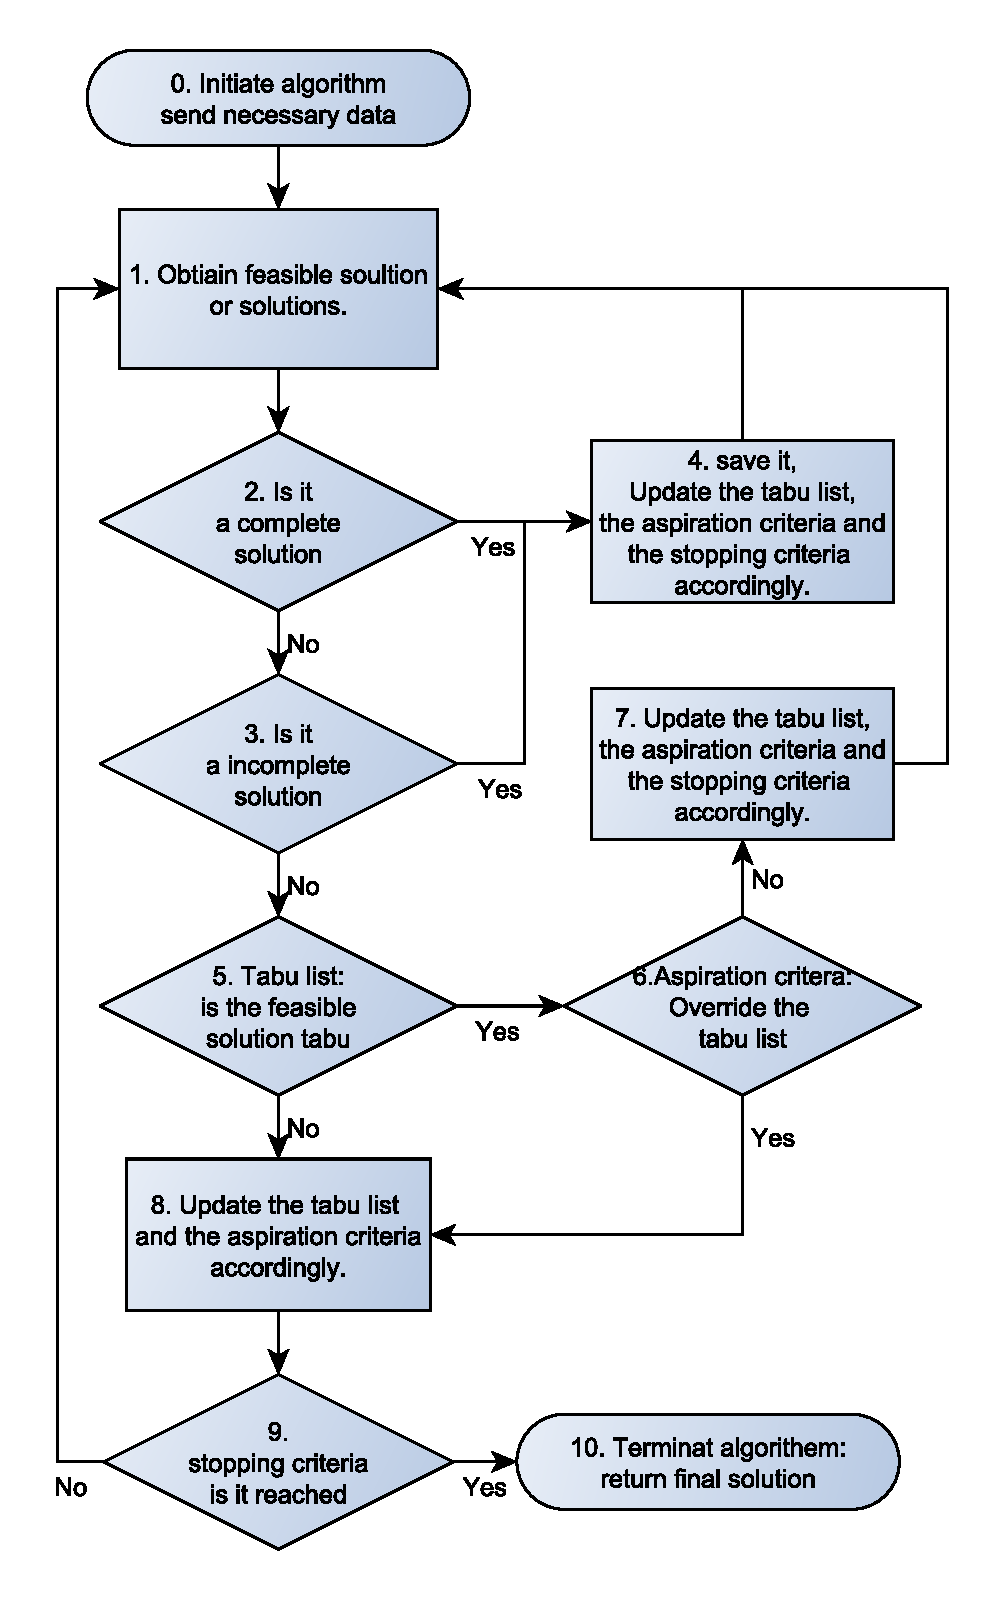
\includegraphics[width=0.75\textwidth,height=0.70\textheight]{chapter_4_methods/ny_generel}
  	\caption[Generic flow chart of tabu algorithm]
  	{Flow chart of tabu algorithm}
	\label{t1}
\end{figure}

\subsection{Development process of the Tabu search algorithm}
The developement process of the tabu search algorithm for our problem will here be described in detail. One of the restrictions of this project was that it had a time shortage due to a deadline. Because of this the alternatives that were easiest to implement was usually prefered. The development process originated from a general flowchart of the algorithm, given in figure \ref{t1}. By following the flow chart, in step one we arrive at the first issue to resolve. The issue of whether to construct a set of feasible solutions, or one single feasible solution at a time. Since the genetic algorithm already had implemented a way of constructing sets of feasible solutions, it was decided to construct one feasible solution at a time.\\
\\
Two alternatives on how to construct this single feasible solution was considered. Either by generating the feasible solution one pursuer step at a time, or by a series of steps. It was decided to construct the feasible solution with one pursuer step at a time. This was a hard decission to make, since both alternatives seemed to yield highly promising but very different algorithms. The implementation of making a series of moves would result in a receding horizon approach, where one had to either  
\begin{itemize}
\item[-]{}Produce a large set of series of moves. Sort these by fitness, then choose one to check against the tabu list and aspiration critera.
\item[-]{}Generate a single series of moves to check against the tabu list and aspiration critera.
\end{itemize}
The implementation of this approach would require that the tabu list and aspiration critera had abilities of a more analysing type. This implied that it would be very difficult to implement within the given time.\\
\\This settled we can now move on to discuss the ideas that form the tabu list. Seven different rules where considered, presented below.
\begin{enumerate}
\item{}For one feasible solution save the past X number of moves for each pursuer and render these moves tabu to be returned to.
\item{}Do not allow moves that results in X number of lost secured tiles.
\item{}Make geometricaly based tabus for critical areas:\vspace{0,1cm}\\
A corridor where the end point can be seen should not be walked down by a pursuer. Also, a region with an obstacle that can be circulated would need two pursuers to be secured. Thus it would be tabu to go about and try to secure it alone. And finaly if one hade a tree like corridor system, going about to solve it would only be allowed with the right amount of pursuers.
\item{} Work togheter. \vspace{0,1cm}\\
Two pursuers never really need to see each other, only share vissible areas. Since this rule is general in its formulation it should be called upon in the aspriation criteria.
\item{} High valued areas \vspace{0,1cm}\\
Tiles walked upon in a complete solution should be given a value bonus. Or implemented differently, tiles not walked upon could be set to be tabu. This is an attempt to incorporate the idea of getting information even from bad, but complete, solutions.
\item{} Low valued areas \vspace{0,1cm}\\
Some tiles that are part of an incomplete solution are probable to be of low interest. Hence these tiles could be given a penalty.
\item{} Treading in secured areas is not probable to yield promising results. Thus this should be given a penalty, or not allowed.
\end{enumerate}

All these tabu rules are to be ranked and given a priority level that would be used in the aspiration criteria. Also many of the tabu rules listed above needed some sort of worst case senario handeling, in order to avoid that the algorithm would freeze.\\
\\We will now discuss the aspiration critera. As understood from the tabu rules presented above a lot is to be incorporated in the aspiration critera. It needs to have the ability of checking whether a tile is of high or low value.

Which in turn means that step 5 in figure \ref{t1} needs a fitness calculation function that would depend on the tile visited and the shape of the feasible solution. Unfortunately this aspiration criteria would need an overwhelming amount of work to implement. Thus this advanced aspiration criteria was rejected for a simpler one. In the end the more simple aspiration criteria only came to be a worst case handling, to avoid the algorithm from freezing. This also means that tabu rules (3), (4), (6) and (7) no longer could be implemented. Tabu rule (5) got simplified to: tiles not walked upon where set to be tabu.\\
\\A comment on tabu rule (5) is that when this rule first was implemented the idea was that X number of past complete solutions were analysed to check which areas had been walked upon at least once, and render the rest tabu. The problem was however that this wasn't strict enough, so X was set to one. Which in turn led to a new problem. The problem that arouse was that the algorithm now, under certain circumstances, was too hasty in returning a final solution, meening that the final solution was of poor quality. This was partially solved by a new stopping criteria and a ``go about it again'' criteria.\\
\\The final version of the algorithm can be viewed in figure \ref{t2} and is also presented in the next section.
\subsection{The Tabu search algorithm for our problem}
In figure \ref{t1} and the previous section a general step by step explanation was made of the tabu search algorithm. In figure \ref{t2}a modified version can be viewed, intended to illustrate the final algorithm. A step by step explanation will be made of figure \ref{t2}. Observe that some functions from to the general algorithm have been removed.\\

There are two elements in the algorithm that affect the convergence. These are the tabu rule (5) and the Best-solution-found-so-far criteria. The tabu rule (5) is explained in the previous section. The Best-solution-found-so-far criteria prohibits the algorithm from searching for solutions longer than the best length found so far. It should be noted that both convergence helping elements depend on the existence of a complete solution. This means that if the algorithm is unlucky in finding the first complete solution, the computational time will rise accordingly. As a side note, this considerable insufficiency might have been avoided with the more advanced aspiration criteria, discussed in section 4.2.2.

\begin{figure}[!h]
\centering
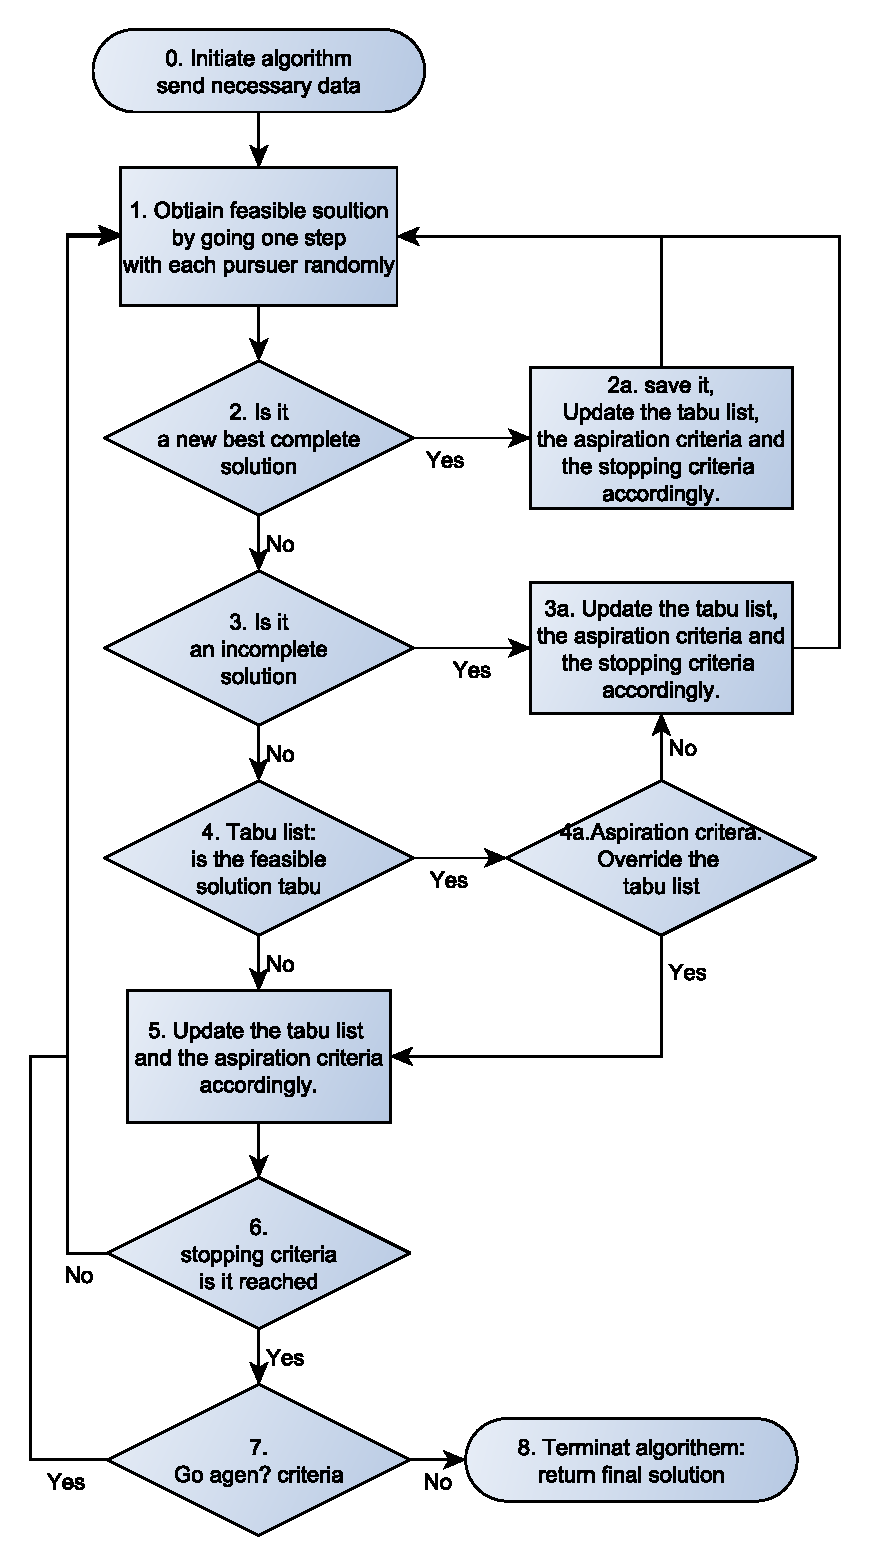
\includegraphics[width=0.75\textwidth,height=0.70\textheight]{chapter_4_methods/ny_Tabu}
\caption[Final algorithm flow chart of tabu algorithm]
{Final algorithm flow chart of tabu algorithm}
\end{figure}

The figure \ref{t2} will now be described in detail.
\begin{enumerate}
\item{}Obtaining feasible solution by going one step with each pursuer randomly. \vspace{0,1cm}\\ 
The input of step 1 is the path taken so far. For the first iteration, or if a completely new feasible solution is to be created, this corresponds only to the starting positions of the pursuers. 
\item{} is it a new best complete solution.
\begin{enumerate}
\item{} if yes the complete solution is saved. An update of the tabu list, the aspiration criteria and the stopping criteria is made accordingly. Then move to 6
\end{enumerate}
\item{} is it an incomplete solution.
\begin{enumerate}
\item{} if yes update the tabu list, the aspiration criteria and the stopping criteria accordingly. Then move back to 1 \vspace{0,1cm}\\
To note her is the change from the general flowchart in figure \ref{t1} to the less sophisticated algorithm. 
\end{enumerate}
\item{} check the feasible solution against the tabu list, is the feasible solution tabu. \vspace{0,1cm}\\
Meaning check tabu rule (1), (2) and (5)
\begin{enumerate}
\item{} if yes the feasible solution is analyzed in the aspiration criteria, whether if the tabu list is to be overrided.
 \begin{enumerate}
\item{} if no, update the tabu list, the aspiration criteria and the stopping criteria accordingly. Then move to 6
\end{enumerate}
\end{enumerate}
\item{} if yes in step 4 or no in step 4a the tabu list, the aspiration criteria and the stopping criteria accordingly. Move to 1
\item{} the stopping criteria. Has it been reached \vspace{0,1cm}\\
Here an evaluation is made whether the algorithm is to be set to cycle through iteration or not. Or if it is to restart with a completely new feasible solution or not. 
Or lastly if the algorithm is to restart with a completely new feasible solution but save the information from tabu rule (5) or not. The last part her was the incorporation of the ``go again criteria’’.
\begin{enumerate}
\item{} if no move to 1
 \begin{enumerate}
\item{} if yes in 6 terminated the algorithm
\end{enumerate}

\subsection{Implementation of the Tabu search algorithm}
In this section two important aspects of the implementation will be discussed. These two are the meaning of the parameter values and obvious shortcomings in the algorithm. With the implementation, a series of parameter values arouse. The parameter values can be divided into four diferent categories.
\begin{enumerate}
\item{} Tabu rule values:
\begin{enumerate}
\item{} save\_past\_X\_number\_of\_steps
\item{} X\_number\_of\_lost\_secured\_tiles
\end{enumerate} 
\item{} Aspiration criteria values:
\begin{enumerate}
\item{} Override\_X\_number\_of\_lost\_secured\_tiles
\item{} Override\_save\_past\_X\_number\_of\_steps
\end{enumerate} 
\item{} Stopping criteria values:
\begin{enumerate}
\item{} Max\_incomplete\_solutions\_ found \_in\_a\_row
\item{} Max\_ equal\_complete\_solutions\_ found\_in\_a\_row
\item{} Max\_allowed\_steps
\end{enumerate} 
\item{} Go again values:
\begin{enumerate}
\item{} Restart\_the\_algorithm\_X\_times
\item{} Restart\_the\_algorithm\_X\_times\_keep\_best\_complete\_solution
\item{} X\_steps\_is\_this\_really\_the\_best\_complete\_solution
\end{enumerate} 
\end{enumerate} 
As can be seen in the list above some of the parameters have strong relations to eachother. These relations will now be explained. \\
Parameter values (1) and (2) are related in such a way so that (2) ensures that (1) does not make the algorithm freeze. \\
Parameter value (4b) and (4c) aims to avoid the algorithm from being to hasty in returning a final solution. This is usually encountered in less difficult enviroments. The Max\_allowed\_steps and Restart\_the\_algorithm\_X\_times tries to tackle the problem of finding the first complete solution. The computational time, and the probability of finding any solution at all, strongly depends on this relation. As discussed lastly in section 4.2.3 the algorithms' computational time will be affected if the first complete solution is found at a late stage in the search. By increasing (3c) the probability of finding any solution should increase. Though this will affect the computational time in a negative way. Both parameter value (3a) and (3b) are to ensure that the algorithm terminates when the search space has been throughly examined in promising areas.
Parameter (3b) is also an indicator of that the the search has converged to a final solution.\\
\\
The implementation of algorithms was made piece by piece. Two of these pieces had known obvious shortcomings. Shortcomings that at the time of implementation were ignored, and due to the lack of time never were treated. These are\\
\begin{enumerate}
\item{} A pursuer cant linger in a tile. \vspace{0,1cm}\\
 An effect of Tabu rule save\_past\_X\_number\_of\_moves.
\item{} large number of precious semi freezes the algorithm\footnote{ The number of large has not been investigated but for 20 pursuers things went south }. \vspace{0,1cm}\\
Also an effect of Tabu rule save\_past\_X\_number\_of\_moves.
\end{enumerate} 
The belief is that both these shortcomings could have been dealt with.

